% Options for packages loaded elsewhere
\PassOptionsToPackage{unicode}{hyperref}
\PassOptionsToPackage{hyphens}{url}
%
\documentclass[
  english,
  man,floatsintext]{apa6}
\usepackage{lmodern}
\usepackage{amsmath}
\usepackage{ifxetex,ifluatex}
\ifnum 0\ifxetex 1\fi\ifluatex 1\fi=0 % if pdftex
  \usepackage[T1]{fontenc}
  \usepackage[utf8]{inputenc}
  \usepackage{textcomp} % provide euro and other symbols
  \usepackage{amssymb}
\else % if luatex or xetex
  \usepackage{unicode-math}
  \defaultfontfeatures{Scale=MatchLowercase}
  \defaultfontfeatures[\rmfamily]{Ligatures=TeX,Scale=1}
\fi
% Use upquote if available, for straight quotes in verbatim environments
\IfFileExists{upquote.sty}{\usepackage{upquote}}{}
\IfFileExists{microtype.sty}{% use microtype if available
  \usepackage[]{microtype}
  \UseMicrotypeSet[protrusion]{basicmath} % disable protrusion for tt fonts
}{}
\makeatletter
\@ifundefined{KOMAClassName}{% if non-KOMA class
  \IfFileExists{parskip.sty}{%
    \usepackage{parskip}
  }{% else
    \setlength{\parindent}{0pt}
    \setlength{\parskip}{6pt plus 2pt minus 1pt}}
}{% if KOMA class
  \KOMAoptions{parskip=half}}
\makeatother
\usepackage{xcolor}
\IfFileExists{xurl.sty}{\usepackage{xurl}}{} % add URL line breaks if available
\IfFileExists{bookmark.sty}{\usepackage{bookmark}}{\usepackage{hyperref}}
\hypersetup{
  pdftitle={Are we all on the same page? Subfield differences in open science practice},
  pdfauthor={Christina Riochios1 \& Jenny L. Richmond1},
  pdflang={en-EN},
  pdfkeywords={keywords},
  hidelinks,
  pdfcreator={LaTeX via pandoc}}
\urlstyle{same} % disable monospaced font for URLs
\usepackage{graphicx}
\makeatletter
\def\maxwidth{\ifdim\Gin@nat@width>\linewidth\linewidth\else\Gin@nat@width\fi}
\def\maxheight{\ifdim\Gin@nat@height>\textheight\textheight\else\Gin@nat@height\fi}
\makeatother
% Scale images if necessary, so that they will not overflow the page
% margins by default, and it is still possible to overwrite the defaults
% using explicit options in \includegraphics[width, height, ...]{}
\setkeys{Gin}{width=\maxwidth,height=\maxheight,keepaspectratio}
% Set default figure placement to htbp
\makeatletter
\def\fps@figure{htbp}
\makeatother
\setlength{\emergencystretch}{3em} % prevent overfull lines
\providecommand{\tightlist}{%
  \setlength{\itemsep}{0pt}\setlength{\parskip}{0pt}}
\setcounter{secnumdepth}{-\maxdimen} % remove section numbering
% Make \paragraph and \subparagraph free-standing
\ifx\paragraph\undefined\else
  \let\oldparagraph\paragraph
  \renewcommand{\paragraph}[1]{\oldparagraph{#1}\mbox{}}
\fi
\ifx\subparagraph\undefined\else
  \let\oldsubparagraph\subparagraph
  \renewcommand{\subparagraph}[1]{\oldsubparagraph{#1}\mbox{}}
\fi
% Manuscript styling
\usepackage{upgreek}
\captionsetup{font=singlespacing,justification=justified}

% Table formatting
\usepackage{longtable}
\usepackage{lscape}
% \usepackage[counterclockwise]{rotating}   % Landscape page setup for large tables
\usepackage{multirow}		% Table styling
\usepackage{tabularx}		% Control Column width
\usepackage[flushleft]{threeparttable}	% Allows for three part tables with a specified notes section
\usepackage{threeparttablex}            % Lets threeparttable work with longtable

% Create new environments so endfloat can handle them
% \newenvironment{ltable}
%   {\begin{landscape}\centering\begin{threeparttable}}
%   {\end{threeparttable}\end{landscape}}
\newenvironment{lltable}{\begin{landscape}\centering\begin{ThreePartTable}}{\end{ThreePartTable}\end{landscape}}

% Enables adjusting longtable caption width to table width
% Solution found at http://golatex.de/longtable-mit-caption-so-breit-wie-die-tabelle-t15767.html
\makeatletter
\newcommand\LastLTentrywidth{1em}
\newlength\longtablewidth
\setlength{\longtablewidth}{1in}
\newcommand{\getlongtablewidth}{\begingroup \ifcsname LT@\roman{LT@tables}\endcsname \global\longtablewidth=0pt \renewcommand{\LT@entry}[2]{\global\advance\longtablewidth by ##2\relax\gdef\LastLTentrywidth{##2}}\@nameuse{LT@\roman{LT@tables}} \fi \endgroup}

% \setlength{\parindent}{0.5in}
% \setlength{\parskip}{0pt plus 0pt minus 0pt}

% \usepackage{etoolbox}
\makeatletter
\patchcmd{\HyOrg@maketitle}
  {\section{\normalfont\normalsize\abstractname}}
  {\section*{\normalfont\normalsize\abstractname}}
  {}{\typeout{Failed to patch abstract.}}
\patchcmd{\HyOrg@maketitle}
  {\section{\protect\normalfont{\@title}}}
  {\section*{\protect\normalfont{\@title}}}
  {}{\typeout{Failed to patch title.}}
\makeatother
\shorttitle{Subfield }
\keywords{keywords\newline\indent Word count: X}
\usepackage{lineno}

\linenumbers
\usepackage{csquotes}
\ifxetex
  % Load polyglossia as late as possible: uses bidi with RTL langages (e.g. Hebrew, Arabic)
  \usepackage{polyglossia}
  \setmainlanguage[]{english}
\else
  \usepackage[shorthands=off,main=english]{babel}
\fi
\ifluatex
  \usepackage{selnolig}  % disable illegal ligatures
\fi
\newlength{\cslhangindent}
\setlength{\cslhangindent}{1.5em}
\newlength{\csllabelwidth}
\setlength{\csllabelwidth}{3em}
\newenvironment{CSLReferences}[2] % #1 hanging-ident, #2 entry spacing
 {% don't indent paragraphs
  \setlength{\parindent}{0pt}
  % turn on hanging indent if param 1 is 1
  \ifodd #1 \everypar{\setlength{\hangindent}{\cslhangindent}}\ignorespaces\fi
  % set entry spacing
  \ifnum #2 > 0
  \setlength{\parskip}{#2\baselineskip}
  \fi
 }%
 {}
\usepackage{calc}
\newcommand{\CSLBlock}[1]{#1\hfill\break}
\newcommand{\CSLLeftMargin}[1]{\parbox[t]{\csllabelwidth}{#1}}
\newcommand{\CSLRightInline}[1]{\parbox[t]{\linewidth - \csllabelwidth}{#1}\break}
\newcommand{\CSLIndent}[1]{\hspace{\cslhangindent}#1}

\title{Are we all on the same page? Subfield differences in open science practice}
\author{Christina Riochios\textsuperscript{1} \& Jenny L. Richmond\textsuperscript{1}}
\date{}


\authornote{

School of Psychology, UNSW

The authors made the following contributions. Christina Riochios: Conceptualization, Methodology, Investigation, Data curation, Visualisation, Formal Analysis, Writing - Original Draft Preparation, Writing - Review \& Editing; Jenny L. Richmond: Conceptualization, Methodology, Formal Analysis, Writing - Original Draft Preparation, Writing - Review \& Editing, Supervision.

}

\affiliation{\vspace{0.5cm}\textsuperscript{1} University of New South Wales}

\abstract{
Although open science has become a popular tool to combat the replication crisis, it is unclear whether the uptake of open science practices has been consistent across the field of psychology. In this study, we utilised open data from a previous study to determine whether data and material sharing, two prominent open science practices, differed as a function of psychological subfield at the distinguished journal, \emph{Psychological Science}. The results showed that Open Data and Open Materials Scores, indicators of data and material sharing, increased from 2014-15 to 2019-20. Of note, articles published in the field of developmental psychology generated considerably lower Open Data and Open Materials Scores, compared to articles in other subfields. These findings are discussed in the context of why developmental psychologists may be slower to adopt open science practices, compared to other researchers, and how journals can more effectively encourage authors to practice open science, across all psychological subfields. As part of our analyses, we also looked at how the awarding of Open Science Badges related to researchers' open science behaviours. Whilst Open Science Badges were closely related to data and material sharing, the usability of the shared data and materials appeared to be questionable. Consequently, we question the value of Open Science Badges in overcoming the replication crisis and propose an alternative open science initiative, that may be more effective.
}



\begin{document}
\maketitle

The field of psychology, like many other scientific disciplines, is currently facing a replication crisis, in which researchers are struggling to replicate existing findings. In 2015, a group of 270 psychological researchers attempted to replicate the findings of 100 psychology experiments. Whilst 97\% of the original studies generated statistically significant findings, only 36\% of the replication attempts were statistically significant. In addition, the replicated effects were, on average, half the size of the original effects (Collaboration, 2015). These findings illustrate the challenge of replicability in psychological research and the pressing need to rectify flawed research practices.

One strategy that has been used to combat the replication crisis within psychology is open science. Open science practices are those that increase the transparency of, and access to, scientific research (Klein et al., 2018). Open data and open materials practices, for example, involve researchers sharing their raw data and experimental materials on publicly accessible online repositories. These practices make it easier for others to replicate the methodology and reproduce the results from published work (Klein et al., 2018).

To encourage researchers to employ open science practices, many psychology journals have implemented incentives, like Open Science Badges. In 2013, the Center for Open Science established three Open Science Badges: Open Data, Open Materials and Preregistered, to acknowledge and reward researchers for their use of open science practices (Center for Open Science, 2021). The Open Data Badge and the Open Materials Badge are awarded when the data and materials that are required to reproduce the methods and results of a study are shared publicly online, whilst the Preregistered Badge is awarded when the design, hypotheses and/or analysis plan are publicly archived prior to data collection. To date, 75 journals (40 in Psychology) have adopted the COS Open Science badges (Center for Open Science, 2021).

At \emph{Psychological Science}, the Association of Psychological Science's flagship journal, Open Science Badges appear to have been successful in encouraging researchers to adopt open science practices. In 2016, Kidwell et al.~coded the frequency of data and material sharing in the 18 months before and after Open Science Badges were implemented at \emph{Psychological Science}. (Kidwell et al., 2016). Kidwell et al.~found that data sharing increased dramatically from 2.5\% prior to badges to 39.4\% following badges. Materials sharing also rose from 12.7\% to 30.3\%. Data and material sharing in control journals, such as the \emph{Journal of Personality and Social Psychology}, which did not award badges, remained low over the same time period (Kidwell et al., 2016). These results led Kidwell et al.~to conclude that Open Science Badges successfully incentivise the uptake of open science practices.

The support for open science continues to grow, however, it is not yet clear whether engagement with open science is consistent across different fields within psychology. Notably, developmental psychology has received significant criticism for its lack of receptivity towards open science. As Figure 1 illustrates, prominent developmental researchers, Prof Michael Frank and Dr.~Jennifer Pfeifer, have labelled the Society for Research in Child Development's (SRCD) open science policy as `weak' and as one that `undervalues openness.' More recently, the Editor-in-Chief of Infant and Child Development, Prof Moin Syed, stated that the uptake of open science within the field of developmental psychology has been `slow and uneven' (Syed, 2020). A survey supporting these viewpoints showed that, on average, 80\% of researchers publishing in \emph{Child Development} felt their institutions failed to provide adequate guidance or financial support for sharing data, (SRCD Task Force on Scientific Integrity and Openness Survey (2017), cited in Gennetian et al., (Gennetian, Tamis-LeMonda, \& Frank, 2020). As such, developmental researchers may be slower to adopt open science practices than those in other psychological disciplines, however, this possibility has yet to be empirically investigated.

FIGURE 1

\begin{figure}
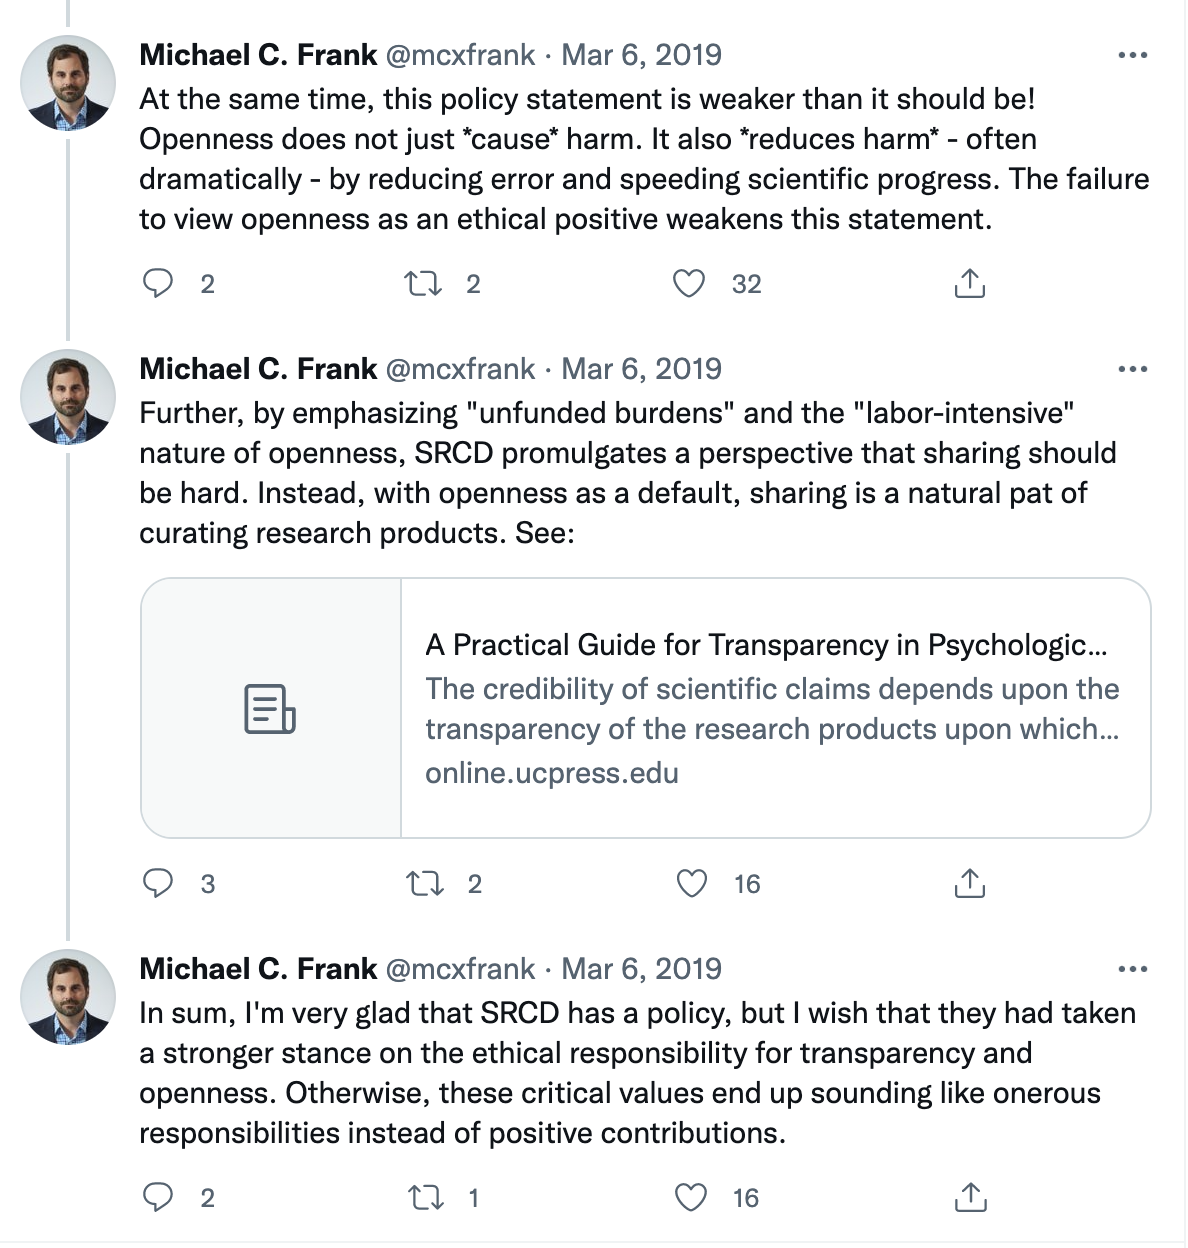
\includegraphics[width=3.96in]{/Users/jenny/Desktop/Desktop - N591/git/same_page/Manuscript/Figure1_mf} \caption{ }\label{fig:unnamed-chunk-1-1}
\end{figure}
\begin{figure}
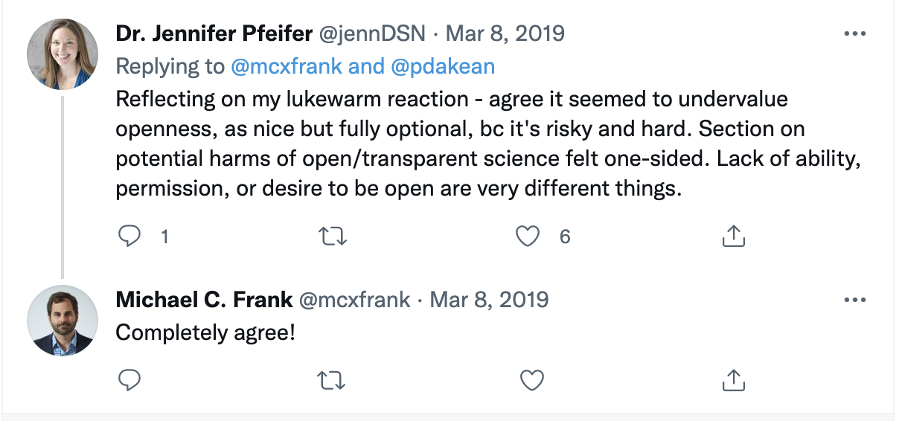
\includegraphics[width=3.01in]{/Users/jenny/Desktop/Desktop - N591/git/same_page/Manuscript/Figure1_jp} \caption{ }\label{fig:unnamed-chunk-1-2}
\end{figure}

Meta-research, the study of research itself, can empirically assess whether developmental psychology is truly behind in the open science movement. Previous investigations, including Kidwell et al. (Kidwell et al., 2016), have revealed that open science incentives can increase the use of open science practices. However, what remains unclear is whether the uptake of open science has been consistent across psychological subfields and sustained over time. To address this research question, we used the open data from the Kidwell et al.~study to examine whether rates of data and material sharing, following the implementation of Open Science Badges at Psychological Science, differed as a function of subfield. In addition, we conducted the same open data and materials coding for articles published in the most recent 18 months (July 2019-Dec 2020) to test whether the badges have continued to be impactful and whether the impact has been consistent across subfields. We were particularly interested in determining whether developmental psychology researchers publishing in Psychological Science engaged with open science practices at the same rate as researchers from other subdomains of psychology. Our methods and analysis plan was preregistered at the Open Science Framework: \url{https://osf.io/3tsmy/}.

\hypertarget{methods}{%
\section{Methods}\label{methods}}

\hypertarget{design}{%
\subsection{Design}\label{design}}

This study had a quasi-experimental design; all articles were systematically assigned to one of seven subfields. Changes in data and material sharing were observed over six-month intervals and were measured using two scores that indexed the transparency of each article's data and materials, respectively.

\hypertarget{sample}{%
\subsection{Sample}\label{sample}}

The sample comprised of all \emph{Psychological Science} articles published between January 2014 and May 2015 (N = 367). As described in the Introduction, Kidwell et al.~(2016) had previously coded these articles to evaluate the openness of their data and materials. To identify how data and material sharing may have changed since 2014-15, our sample also included all \emph{Psychological Science} articles that were published between July 2019 and December 2020 (N = 242). Non-empirical articles that did not contain an experiment or analysis, including editorials, commentaries, replies, corrigenda, errata and retractions, were excluded from our analysis. After filtering out these non-empirical articles from the sample, 322 articles published between 2014-15 and 193 articles published between 2019-20, remained.

\hypertarget{materials}{%
\subsection{Materials}\label{materials}}

To assess the transparency of each article's data and materials, Kidwell et al.~(2016) employed a systematic coding system (see Appendix A) comprising of a series of variables, defined in Appendix B. We downloaded the data Kidwell et al.~coded from their OSF repository (\url{https://osf.io/rfgdw/}) and filtered the dataset to only include data from \emph{Psychological Science} articles published between January 2014 and May 2015.
In addition to the variables Kidwell et al.~coded, we also coded for whether the authors of each article specified the type of software that was used to analyse their data. When authors' identify their analysis software, the analysis procedure can be easier to follow, and the chance of others' successfully reproducing the study's data, may increase (National Academics of Sciences Engineering and Medicine, 2019). Thus, although Kidwell et al.~did not code for analysis software, it is an important variable to consider when assessing the transparency of a study's data. We coded for two variables to account for analysis software; first, whether the article specified their analysis software or not, and second, which type of analysis software had been specified (e.g., R, JASP, SPSS etc.).
To code the articles that were published between July 2019 and December 2020, we used the same amended version of the Kidwell et al.~coding system, which included the two additional variables that accounted for the article's analysis software.

To assign all the articles to a subfield, we used the coding system outlined in Appendix D. Articles were assigned to one of seven psychological subfields: Developmental Psychology, Social Psychology, Cognition, Perception, Health Psychology, Cognitive Neuroscience and Behavioural Neuroscience. We identified these seven subfields as those that the vast majority of \emph{Psychological Science} articles fall into, after thoroughly reviewing the journal's website. The variables that we coded are defined in Appendix C. As an example, one of the variables we coded was the age of the participants recruited in the study. Distinguishing participants from children to adults allowed us to assign articles to the Developmental Psychology subfield.

Prior to data collection, each member of the coding team coded five trial articles. The trial articles aimed to confirm coders' understanding of the coding process prior to them coding the target articles. These trial articles were \emph{Psychological Science} articles originally coded by Mallory Kidwell, the primary investigator in the Kidwell et al.~(2016) study. Kidwell's coding acted as a `gold standard' to which coders' responses were compared. The senior coder in the current study generated the gold standard for the variables that weren't included in the Kidwell et al.~coding system. The trial articles varied in the transparency of their data and materials, and therefore, exposed coders to a representative range of coding outcomes.

The coding team coded both the trial and target articles via a Qualtrics survey, containing a series of multiple-choice questions. The questions were structured in an `if-then' manner, with consecutive questions only being asked if coders provided certain answers to the questions prior. For example, according to the coding system in Appendix D, coders were only asked about the participants' age, if they had specified that the participants in the study were `Humans' as opposed to `Animals.'

\hypertarget{procedure}{%
\subsection{Procedure}\label{procedure}}

After the investigation had been approved by the UNSW Human Research Ethics Advisory Panel, we assembled a team of volunteer coders, comprising of undergraduate UNSW psychology students. Once the coders coded the five trial articles and the senior coder was confident that each coder understood how to code all the variables correctly, the coders were provided access to the target set of articles and were allowed to begin coding.
Analysis procedure
After all articles had been coded, we imported the data from Qualtrics into the software environment, R (R Core Team, 2021). For the articles that were published between 2014-15, we combined the newly collected data with the relevant Kidwell et al.~(2016) data. Each article, across both the 2014-15 and 2019-20 datasets, was assigned to one of the seven psychological subfields, and received an Open Data and Open Materials Score. A study's Open Data Score indexed the extent to which its data were transparent, whilst the Open Materials Score indexed the extent to which the article's materials were transparent. Therefore, to calculate the scores, we weighted each coded variable according to how much it improved the transparency of the article's data and materials, respectively. There were three levels of transparency: low-level transparency variables received a value of 1, moderate-level transparency variables received a value of 2 and high-level transparency variables received a value of 5 (see Table 1). We summed these scores so that each article received an Open Data Score out of a possible 25 and an Open Materials Score out of a possible 19. Higher scores were indicative of a higher level of transparency.

\hypertarget{insert-table-1-here}{%
\section{INSERT TABLE 1 HERE}\label{insert-table-1-here}}

\emph{Reliability} After the 2014-15 sample of articles had been coded, the senior coder randomly selected 25 empirical articles from the dataset (8\% of the empirical sample), ensuring that an equal number had been coded by each coder (n = 5), and double-coded these articles to generate a gold standard for subfield assignment. Using the `kappa2' function from the `irr' package in R (Gamer et al., 2019), we ran a Cohen's Kappa reliability analysis for subfield assignment, to assess how well the coders' coding matched the gold standard.
For the 2019-20 sample of articles, the senior coder similarly selected 25 articles from the empirical sample (13\%) and double-coded these articles to produce a gold standard. Each article received a Total Openness Score, representing the sum of the article's Open Data and Open Materials Score. To assess reliability, we used the `icc' function from the `irr' package in R to generate an intraclass correlation coefficient (ICC) from the coders' Total Openness Scores and the gold standard's (Gamer et al., 2019). The `tolerance' level was set at five Total Openness points; where scores fell within a five-point range of each other, they were considered to be equivalent.
As a secondary measure of inter-rater reliability, we also calculated the percent agreement between the gold standard and coders' responses, for both the 2014-15 and 2019-20 datasets.

\hypertarget{data-analysis}{%
\subsection{Data analysis}\label{data-analysis}}

We used R {[}Version 4.0.3; R Core Team (2020){]} and the R-packages \emph{afex} {[}Version 1.0.1; Singmann, Bolker, Westfall, Aust, and Ben-Shachar (2021){]}, \emph{apa} {[}Version 0.3.3; Gromer (2020); Aust and Barth (2020){]}, \emph{dplyr} {[}Version 1.0.7; Wickham, François, Henry, and Müller (2021){]}, \emph{forcats} {[}Version 0.5.1; Wickham (2021a){]}, \emph{ggeasy} {[}Version 0.1.3; Carroll, Schep, and Sidi (2021){]}, \emph{gghalves} {[}Version 0.1.1; Tiedemann (2020){]}, \emph{ggplot2} {[}Version 3.3.5; Wickham (2016){]}, \emph{ggsignif} {[}Version 0.6.3; Constantin and Patil (2021){]}, \emph{goodshirt} {[}Version 0.2.2; Gruer (2021){]}, \emph{here} {[}Version 1.0.1; Müller (2020){]}, \emph{janitor} {[}Version 2.1.0; Firke (2021){]}, \emph{lme4} {[}Version 1.1.27.1; Bates, Mächler, Bolker, and Walker (2015){]}, \emph{Matrix} {[}Version 1.3.4; Bates and Maechler (2021){]}, \emph{papaja} {[}Version 0.1.0.9997; Aust and Barth (2020){]}, \emph{patchwork} {[}Version 1.1.1; Pedersen (2020){]}, \emph{purrr} {[}Version 0.3.4; Henry and Wickham (2020){]}, \emph{readr} {[}Version 2.0.1; Wickham and Hester (2021){]}, \emph{report} {[}Version 0.3.5; Makowski, Ben-Shachar, Patil, and Lüdecke (2021){]}, \emph{stringr} {[}Version 1.4.0; Wickham (2019){]}, \emph{tibble} {[}Version 3.1.4; Müller and Wickham (2021){]}, \emph{tidyr} {[}Version 1.1.3; Wickham (2021b){]}, and \emph{tidyverse} {[}Version 1.3.1; Wickham et al. (2019){]} for all our analyses.

\emph{Confirmatory Analyses} Four Analysis of Variance (ANOVA) analyses were run to investigate differences in Open Data and Open Materials Scores, separately, across the 2014-15 and 2019-20 datasets. In each analysis, we tested for a main effect of time, measured over three six-month intervals, and subfield. To ensure that there was a comparable number of articles in each subfield group, we combined Cognitive Neuroscience, Behavioural Neuroscience, Health Psychology and Perception into a single `Other' category. As a result, a total of four subfield groups were included in our analysis: Developmental Psychology, Social Psychology, Cognition and Other. In each ANOVA analysis, we also included a time by subfield interaction to test whether the changes in Open Data and Open Materials Scores over time, differed as a function of subfield. We measured effect sizes in terms of generalised eta squared (ges). For each ANOVA result, the ges represented the proportion of variance that was accounted for by the variable of interest (Olejnik \& Algina, 2003).
To identify how the transparency of data and materials had changed between 2014-15 and 2019-20, we ran two additional ANOVA analyses, which tested for the same main effects and interaction effect as the previous ANOVAs. The time effect had two levels: 2014-15 and 2019-20.

\emph{Exploratory Analyses} After scoring the data, we noticed that a large proportion of articles had received an Open Data and Open Materials Score of zero. This observation led us to generate two raincloud plots that illustrated the distribution of Open Data and Open Materials Scores across 2019-20, respectively. Raincloud plots visualise the distribution of scores in a dataset by showing the concentration of subjects at each level of the dependent measure. In our case, where the plot was wider, the concentration of articles that received the corresponding Open Data or Open Materials Score, was higher. The two raincloud plots illustrated the distribution of scores per subfield.

In addition to analysing Open Data and Open Materials Scores, we were also interested in identifying how the awarding of Open Science Badges related to researchers' data and materials sharing practices. To generate two corresponding figures, we filtered the 2019-20 dataset to only include the articles that had received an Open Data Badge and an Open Materials Badge, respectively. We then plotted the percentage of these articles that met a series of data and materials sharing criteria, described in the Results section below.

\emph{Preregistration} We preregistered our aims, hypotheses, design, and planned analysis procedure for the study at the OSF: \url{https://osf.io/3tsmy/}. Whilst we attempted to follow each of the proposed procedures as closely as possible, we made one notable modification. Namely, we chose not to normalise the Open Data and Open Materials Scores (so that they were both out of 100). Since our study was focussed on measuring subfield differences and changes over time, within each type of score, rather than comparing the differences between the two scores, we ultimately realised that normalising the scores was not necessary. All the materials, data and analysis scripts from the study can be accessed via the OSF: \url{https://osf.io/z8b7j/}.

\hypertarget{results}{%
\section{Results}\label{results}}

We first used the open data from Kidwell et al., (2016) and analysed whether open data and open materials scores improved across the 2014-2015 period and differed by subfield. As illustrated in Figure 2A, for open data scores the main effect of subfield, \(F(3, 310) = 2.23\), \(\mathit{MSE} = 41.51\), \(p = .085\), \(\hat{\eta}^2_G = .021\), was not significant, indicating that during the period immediately following the badge policy change, open data scores were uniformly low across subfields. There was a significant main effect of time period, \(F(2, 310) = 11.29\), \(\mathit{MSE} = 41.51\), \(p < .001\), \(\hat{\eta}^2_G = .068\), however, the improvement in open data scores over this 18 month period did not differ as a function of subfield, \(F(6, 310) = 1.57\), \(\mathit{MSE} = 41.51\), \(p = .157\), \(\hat{\eta}^2_G = .029\).

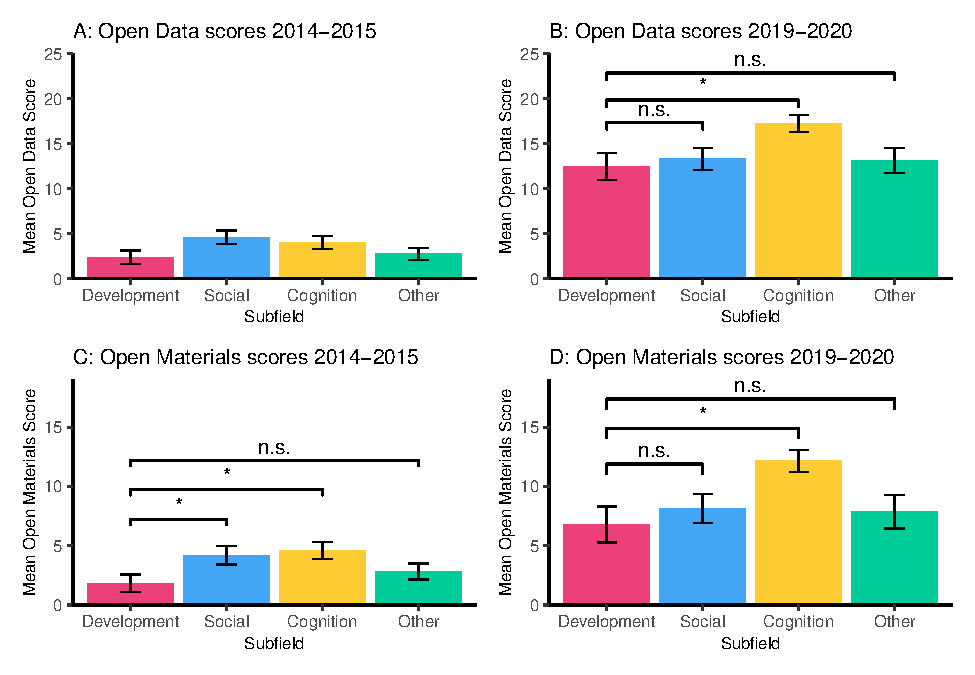
\includegraphics{icd_special_issue_files/figure-latex/unnamed-chunk-2-1.pdf}
\emph{Figure 2}: Mean open data and open materials scores for articles published in \emph{Psychological Science} between 2014-2015 and 2019-2020 as a function of subfield.

Across the 2019-2020 period, open data scores also increased significantly , \(F(2, 181) = 3.68\), \(\mathit{MSE} = 70.92\), \(p = .027\), \(\hat{\eta}^2_G = .039\), and differed by subfield, \(F(3, 181) = 3.31\), \(\mathit{MSE} = 70.92\), \(p = .021\), \(\hat{\eta}^2_G = .052\). When we compared the open data scores from papers published in developmental psychology to each of the other subfield categories (Figure 2B), we found that papers in developmental psychology had significantly lower open data scores (\emph{M} = 12.50, \emph{SD} = 8.83) than papers in cognition (\emph{M} = 17.23, \emph{SD} = 7.37), \(t(58.75) = -2.65\), \(p = .010\), but did not differ from papers published in social psychology (\emph{M} = 13.32, \emph{SD} = 9.17), \(t(71.68) = -0.42\), \(p = .675\) or those that fell into the other category (\emph{M} = 13.15, \emph{SD} = 9.07), \(t(71.12) = -0.31\), \(p = .756\). There was no significant time by subfield interaction, \(F(6, 181) = 1.11\), \(\mathit{MSE} = 70.92\), \(p = .358\), \(\hat{\eta}^2_G = .035\).

For open materials scores across 2014-2015, there were significant main effects of both subfield, \(F(3, 310) = 4.03\), \(\mathit{MSE} = 32.16\), \(p = .008\), \(\hat{\eta}^2_G = .038\), and time period, \(F(2, 310) = 4.74\), \(\mathit{MSE} = 32.16\), \(p = .009\), \(\hat{\eta}^2_G = .030\) (see Figure 2C). Papers in developmental psychology had lower open materials scores (\emph{M} = 1.82, \emph{SD} = 6.02) than those in both social (\emph{M} = 4.19, \emph{SD} = 7.34), \(t(153.62) = -2.75\), \(p = .007\), and cognition (\emph{M} = 4.59, \emph{SD} = 7.07), \(t(153.74) = -3.20\), \(p = .002\), but developmental open materials scores did not differ from papers allocated to the other subfield category (\emph{M} = 2.83, \emph{SD} = 5.84), \(t(137.95) = -1.19\), \(p = .236\). The interaction between time period and subfield, \(F(6, 310) = 0.85\), \(\mathit{MSE} = 32.16\), \(p = .530\), \(\hat{\eta}^2_G = .016\), was not statistically significant.

As illustrated in Figure 2D, there were also subfield differences in open materials scores during the 2019-2020 period, \(F(3, 181) = 5.24\), \(\mathit{MSE} = 53.87\), \(p = .002\), \(\hat{\eta}^2_G = .080\). Consistent with open data scores, papers published in developmental psychology had significantly lower open materials scores (\emph{M} = 6.79, \emph{SD} = 8.83) than papers published in cognition, (\emph{M} = 6.79, \emph{SD} = 8.83), \(t(61.36) = -3.45\), \(p = .001\), however, open materials scores did not differ between developmental and social psychology (\emph{M} = 6.79, \emph{SD} = 8.83), \(t(68.36) = -0.84\), \(p = .406\), or between developmental psychology and the other subfield category (\emph{M} = 6.79, \emph{SD} = 8.83), \(t(70.45) = -0.62\), \(p = .539\). There were no additional changes in open materials scores across the time period between mid-2019 and the end of 2020, \(F(2, 181) = 0.37\), \(\mathit{MSE} = 53.87\), \(p = .694\), \(\hat{\eta}^2_G = .004\), and differences in subfield did not vary over time, \(F(6, 181) = 0.48\), \(\mathit{MSE} = 53.87\), \(p = .822\), \(\hat{\eta}^2_G = .016\).

It is clear that since the introduction of open science badges in 2014, papers published in \emph{Psychological Science} have become more open over time and that most recently, developmental psychology has lagged behind some, but not all, subfields. To determine whether the rate of improvement from 2014-2015 through 2019-2020 differed significantly by subfield, we combined the data across the two coded time periods and looked for subfield by time interactions in both open data and open materials scores. As illustrated in Figure 3, there was no evidence that the magnitude of improvement over time differed by subfield for either both open data scores \(F(3, 507) = 2.28\), \(\mathit{MSE} = 55.28\), \(p = .078\), \(\hat{\eta}^2_G = .013\) or open materials scores \(F(3, 507) = 2.07\), \(\mathit{MSE} = 40.21\), \(p = .103\), \(\hat{\eta}^2_G = .012\).

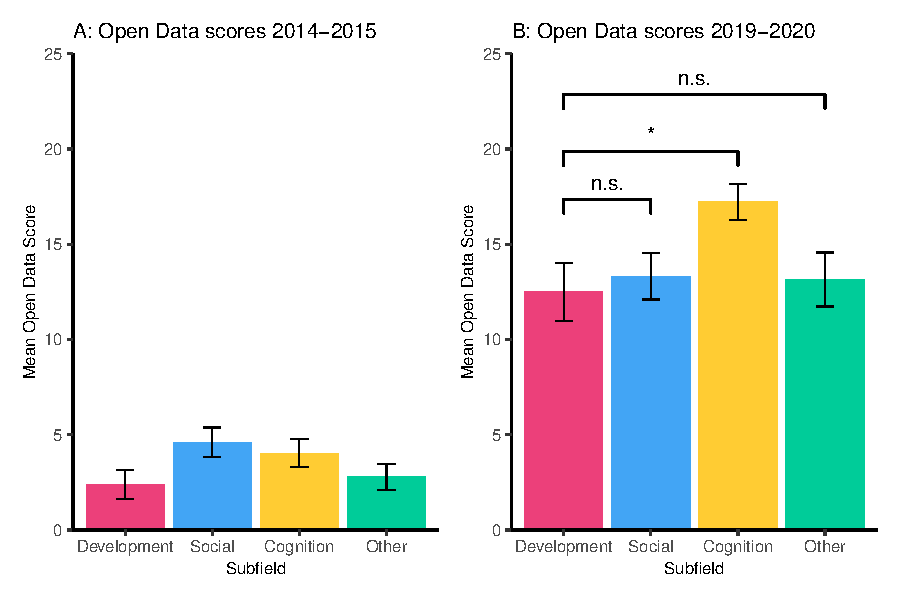
\includegraphics{icd_special_issue_files/figure-latex/unnamed-chunk-3-1.pdf}
\emph{Figure 3}: Mean open data and open materials scores for articles published in \emph{Psychological Science} as a function of subfield and time period.

\hypertarget{exploratory}{%
\section{EXPLORATORY}\label{exploratory}}

Our confirmatory analyses showed that on average, open data and materials scores for papers published in \emph{Psychological Science} have increased markedly across all subfields, however, it is clear that scores within each subfield varied widely. To capture changes in variability over time, we used raincloud plots (\textbf{allen2019raincloud?}) to represent the distribution of open data and materials scores across subfields. Figure 4 illustrates that in 2014-2015, across all subfields, most open data and open materials scores were low, with between 70-80\% of papers receiving scores less than 5. In contrast in 2019-2020, the distribution is bimodal. The majority of papers score on the upper half of the scale, however, there are still one third of papers published that receive scores less than 5.

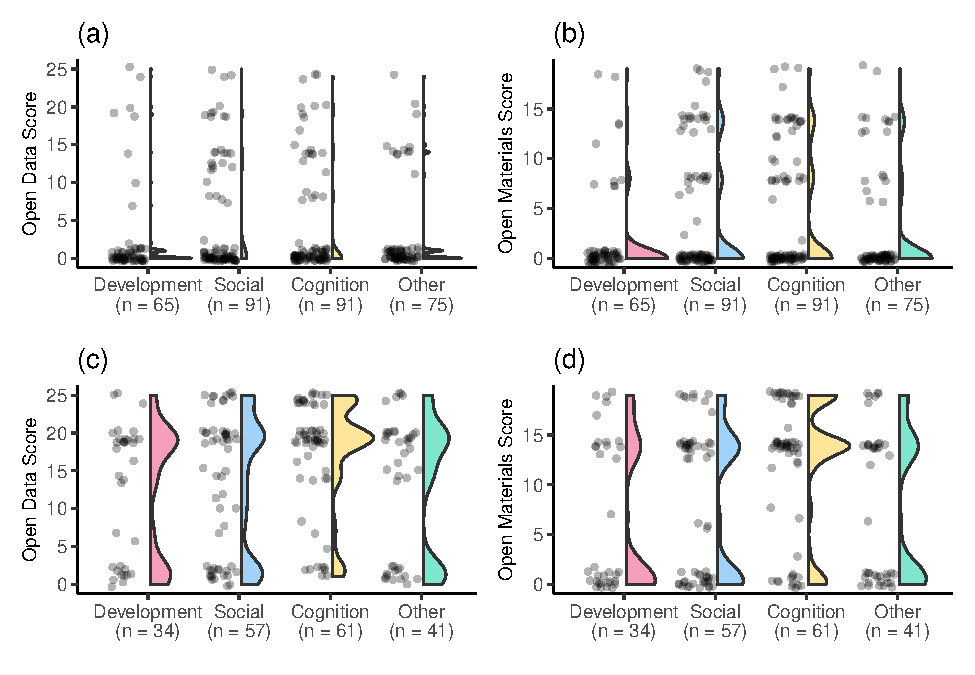
\includegraphics{icd_special_issue_files/figure-latex/rain_combo-1.pdf}
\textbf{Figure 4}: Distribution of open data and open materials scores earned by articles published in \emph{Psychological Science} as a function of subfield

We were surprised how few articles received very high open data and materials scores even in 2019-2020. In order to receive very high scores, article authors needed to engage in behaviours that make shared resources most useful (i.e.~sharing data with a accompanying codebook and analysis script) and we particularly interested in how common this kind of metadata sharing was among papers that had earned an Open Data or Open Materials Badge. To produce Figure 5, we filtered articles published within the 2019-20 window for those that were awarded open data and materials badges and then plotted the proportion of those articles that shared codebooks and scripts along with complete data. It is clear from the Figure that whie the vast majority of papers earning an open data badge had complete data available, only half shared a codebook and X\% included a analysis script. Similarly for open materials, most articles earning a badge shared raw materials on an open repository but a relatively small percentage of articles also shared an script and/or detailed explanation of how to use the materials in a replication study.

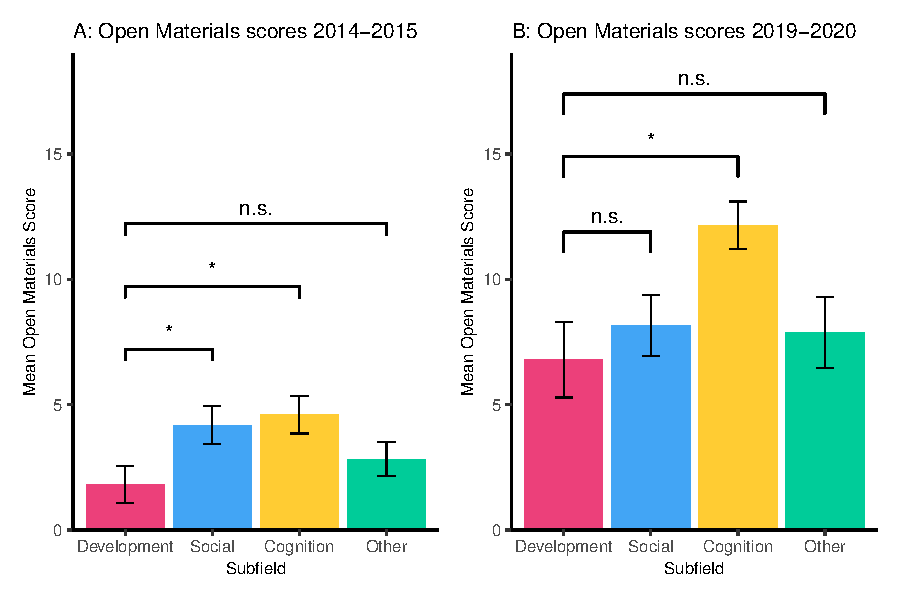
\includegraphics{icd_special_issue_files/figure-latex/unnamed-chunk-4-1.pdf}
\emph{Figure 5} Badges plot

\hypertarget{discussion}{%
\section{Discussion}\label{discussion}}

In the past few years, there has been concern from some academics that developmental psychology was lagging behind in its use of open science practices, compared to other psychological subfields. The results of the current study provide empirical support for this idea. Across both 2014-15 and 2019-20, developmental psychology articles published in \emph{Psychological Science} had significantly lower Open Materials Scores than cognitive psychology articles. In 2019-20, developmental psychology articles also hadlower Open Data Scores relative to cognition articles.

There are several factors that may be contributing to lower open data and open materials scores in developmental psychology. Notably, practicing open science may pose a greater reputational risk to developmental scientists compared to researchers from other subdisciplines (Gilmore et al., 2020). Participants in developmental research are temperamental and unpredictable, which makes it difficult for researchers to stick to strict experimental protocols (Peterson, 2016). For example, if a child is getting fussy, the experimenter may deviate from the experimental protocol and allow the parent to complete the paradigm with them (Slaughter \& Suddendorf, 2007). These ``off-protocol'' decisions make experimental protocols difficult to replicate and add noise to experimental data (Peterson, 2016). Researchers may be reluctant to share data and materials online, out of fear that they will be criticised for a lack of scientific rigor, and that their reputation may be harmed (Gilmore et al., 2020). It is possible that the perceived risks of data and material sharing in developmental psychology may impact openness and transparency

The scarcity of data in developmental psychology may further impede data sharing. Developmental scientists usually recruit their participants from off-campus locations (Peterson, 2016) making recruitment a time consuming and expensive process and sample sizes generally small (Davis-Kean \& Ellis, 2019). In contrast, cognition researchers are typically able to recruit large samples of participants on campus or from online platforms (Benjamin, 2019). According to the law of supply and demand, which asserts that rare commodities are more highly valued (Steuart, 1767), developmental researchers may place greater value on their data than researchers in other subfields. Given that willingness to share decreases as the value of an item increases (Hellwig et al., 2015), it is possible that the nature of developmental data reduces the likelihood that developmental scientists will share compared to other psychological subfields, such as cognition.

Finally, the methods that developmental psychologists use may make it particularly difficult to share materials openly. As Peterson (2016) reports, in developmental studies, experimental stimuli are typically constructed by hand and are set up manually by research assistants. The physical nature of these experimental paradigms may make them more difficult, and sometimes impossible, to share online. In contrast, computer-based experimental paradigms are becoming increasingly popular in the fields of cognition and social psychology. These paradigms, which can be automated and run online, make it relatively easy to upload materials to online repositories (Paxton \& Tullett, 2019). Therefore, the types of materials researchers employ may explain why developmental psychologists may be less likely to share materials than researchers in other subfields.

Although developmental psychology appears to be lagging behind other subfields, there is cause for optimism. Open data and materials scores for developmental psychology articles published in \emph{Psychological Science} improved from 2014 to 2020 at the same rate as articles in other subfields. It seems that developmental psychology researchers, at least those who are looking to publish in \emph{Psychological Science}, are keeping up with their colleagues and becoming more and more likely to adopt open data and open materials into their research workflow.

Although open data and materials practices are becoming more common, the current findings highlight the significant progress that is yet to be made in the open science movement across psychology. We were surprised to see that in 2019-20, Open Data and Open Materials Scores were bimodally distributed (see Figure X), with a large proportion of articles receiving extremely low scores. In addition, very few articles were awarded the highest possible Open Data and Open Materials Score, indicating that even when data and materials were shared, they were often not accompanied by the metadata that is necessary for data and materials to be usable. These underwhelming results suggest that researchers may need further convincing of how the benefits of open and transparent research practice, both personally and for the field, outweigh the time and effort required to change research workflow (Markowetz, 2015).

point re personal benefit was here

Like all open science incentives, Open Science Badges are not an end to themselves; although the aim is to increase the transparency of research methods, the ultimate goal is to improve the replicability. The results of the current study question the success of Open Science Badges in achieving this goal at \emph{Psychological Science}. Whilst a high proportion of the articles that received an Open Data and Open Materials Badge across 2014-15 and 2019-20, had data and materials that were locatable and complete, a much smaller percentage shared a codebook, analysis script and/or explanation of the materials. Roche et al.~(2015) suggests that without corresponding metadata, open data and open materials may may be not be usable, both for the purpose of reproducing the findings of a particular study and conducting novel research (Roche et al., 2015). Open Science Badges may incentivise researchers to share their data and materials, but if they do not increase the availability of metadata, then their value in overcoming the replication crisis, remains debatable.

Our results also raise concerns about how well Open Science Badges criteria are adhered to, in practice. According to the COS, Open Data Badges can only be awarded if a `data dictionary' such as a codebook, or other related metadata that would allow other researchers to reproduce the analyses and results, is available with the data (Center for Open Science, 2013a). Similarly, for articles to be awarded an Open Materials Badge, the authors must provide a sufficiently detailed explanation of how the materials were used in the study, and how they can be reproduced, if they can't be shared digitally (Center for Open Science, 2013b). We found that only 45\% of the articles that were awarded an Open Data Badge in 2019-20, shared a codebook, and only 35\% of those awarded an Open Materials Badge provided an explanation of their materials. These results not only suggest that a very small proportion of the articles that received an Open Data and/or Open Materials Badge were truly deserving of one, but they also show that the criteria for Open Science Badges may be applied inconsistently. Further research is required to identify whether this issue is specific to \emph{Psychological Science}, or if it is a broader issue observed across all journals that award Open Science Badges. In any case, the potentially inconsistent application of the criteria for Open Science Badges questions how valid and reliable they are as indicators of transparency and usability.

Where to from here? It is clear that Open Badges have has an impact on author behaviour at Psychological Science and that there is work to do within developmental psychology. \emph{Psychological Science} was ideally suited for our open science subfield comparison due to its broad publishing scope. However, because \emph{Psychological Science} implemented Open Science Badges, and is one of psychology's top tier journals, publishing only a very small subset of high quality and novel research articles, it is unclear whether the results from the current study are reflective of the field of psychology as whole. Future meta-research should focus on open science practices across a broader range of developmental outlets to assess whether it is the badges per se, or a broader shift in research workflow that has resulted in improved transparency at \emph{Psychological Science}.

Although Open Badges may encourage authors to be more open in their research, it is possible that they are rewarding researchers for doing the bear minimum, and not actually pushing the field toward a more replicable science. Perhaps journals should consider employing an open science scoring system, instead. Such a system (see Yang et al., 2020; Hartshorne \& Schachner, 2012 for related examples) would involve psychology journals awarding each article they publish a ``Reproduciblity Score'' that indexes the likelihood of the study's findings being successfully reproduced based on the transparency of its data and materials. To maximise objectivity and to minimise time costs, an automated algorithm would generate each article's Reproducibility Score (Altmejd et al., 2019; Yang et al., 2020). Future research should test whether compared to Open Science Badges, scores may be a more precise and meaningful indicator of transparency and potential replicaablity.

To conclude, the present study provides support for the existence of subfield differences in the uptake of open science practices, across the field of psychology. Whilst the findings indicated that researchers' use of open science practices have increased since \emph{Psychological Science} introduced Open Science Badges in 2014, there appears to be considerable progress yet to be made. Although Open Science Badges do not appear to be as valuable in overcoming the replication crisis as they seem, an open science scoring system may provide a promising alternative. Overall, we hope that the results of the study enhance the way open science is endorsed and applied across psychological subfields.

\newpage

\hypertarget{references}{%
\section{References}\label{references}}

\begingroup
\setlength{\parindent}{-0.5in}
\setlength{\leftskip}{0.5in}

\hypertarget{refs}{}
\begin{CSLReferences}{1}{0}
\leavevmode\hypertarget{ref-R-papaja}{}%
Aust, F., \& Barth, M. (2020). \emph{{papaja}: {Create} {APA} manuscripts with {R Markdown}}. Retrieved from \url{https://github.com/crsh/papaja}

\leavevmode\hypertarget{ref-R-Matrix}{}%
Bates, D., \& Maechler, M. (2021). \emph{Matrix: Sparse and dense matrix classes and methods}. Retrieved from \url{https://CRAN.R-project.org/package=Matrix}

\leavevmode\hypertarget{ref-R-lme4}{}%
Bates, D., Mächler, M., Bolker, B., \& Walker, S. (2015). Fitting linear mixed-effects models using {lme4}. \emph{Journal of Statistical Software}, \emph{67}(1), 1--48. \url{https://doi.org/10.18637/jss.v067.i01}

\leavevmode\hypertarget{ref-R-ggeasy}{}%
Carroll, J., Schep, A., \& Sidi, J. (2021). \emph{Ggeasy: Easy access to 'ggplot2' commands}. Retrieved from \url{https://CRAN.R-project.org/package=ggeasy}

\leavevmode\hypertarget{ref-open2015estimating}{}%
Collaboration, O. S. (2015). Estimating the reproducibility of psychological science. \emph{Science}, \emph{349}(6251).

\leavevmode\hypertarget{ref-R-ggsignif}{}%
Constantin, A.-E., \& Patil, I. (2021). {ggsignif}: R package for displaying significance brackets for {'ggplot2'}. \emph{PsyArxiv}. \url{https://doi.org/10.31234/osf.io/7awm6}

\leavevmode\hypertarget{ref-R-janitor}{}%
Firke, S. (2021). \emph{Janitor: Simple tools for examining and cleaning dirty data}. Retrieved from \url{https://CRAN.R-project.org/package=janitor}

\leavevmode\hypertarget{ref-gennetian2020advancing}{}%
Gennetian, L. A., Tamis-LeMonda, C. S., \& Frank, M. C. (2020). Advancing transparency and openness in child development research: opportunities. \emph{Child Development Perspectives}, \emph{14}(1), 3--8.

\leavevmode\hypertarget{ref-R-apa}{}%
Gromer, D. (2020). \emph{Apa: Format outputs of statistical tests according to APA guidelines}. Retrieved from \url{https://CRAN.R-project.org/package=apa}

\leavevmode\hypertarget{ref-R-goodshirt}{}%
Gruer, A. (2021). \emph{Goodshirt: R client for the good place quotes API}.

\leavevmode\hypertarget{ref-R-purrr}{}%
Henry, L., \& Wickham, H. (2020). \emph{Purrr: Functional programming tools}. Retrieved from \url{https://CRAN.R-project.org/package=purrr}

\leavevmode\hypertarget{ref-kidwell2016badges}{}%
Kidwell, M. C., Lazarević, L. B., Baranski, E., Hardwicke, T. E., Piechowski, S., Falkenberg, L.-S., \ldots{} others. (2016). Badges to acknowledge open practices: A simple, low-cost, effective method for increasing transparency. \emph{PLoS Biology}, \emph{14}(5), e1002456.

\leavevmode\hypertarget{ref-klein2018practical}{}%
Klein, O., Hardwicke, T. E., Aust, F., Breuer, J., Danielsson, H., Mohr, A. H., \ldots{} others. (2018). A practical guide for transparency in psychological science. \emph{Collabra: Psychology}, \emph{4}(1).

\leavevmode\hypertarget{ref-R-report}{}%
Makowski, D., Ben-Shachar, M. S., Patil, I., \& Lüdecke, D. (2021). Automated results reporting as a practical tool to improve reproducibility and methodological best practices adoption. \emph{CRAN}. Retrieved from \url{https://github.com/easystats/report}

\leavevmode\hypertarget{ref-R-here}{}%
Müller, K. (2020). \emph{Here: A simpler way to find your files}. Retrieved from \url{https://CRAN.R-project.org/package=here}

\leavevmode\hypertarget{ref-R-tibble}{}%
Müller, K., \& Wickham, H. (2021). \emph{Tibble: Simple data frames}. Retrieved from \url{https://CRAN.R-project.org/package=tibble}

\leavevmode\hypertarget{ref-R-patchwork}{}%
Pedersen, T. L. (2020). \emph{Patchwork: The composer of plots}. Retrieved from \url{https://CRAN.R-project.org/package=patchwork}

\leavevmode\hypertarget{ref-R-base}{}%
R Core Team. (2020). \emph{R: A language and environment for statistical computing}. Vienna, Austria: R Foundation for Statistical Computing. Retrieved from \url{https://www.R-project.org/}

\leavevmode\hypertarget{ref-R-afex}{}%
Singmann, H., Bolker, B., Westfall, J., Aust, F., \& Ben-Shachar, M. S. (2021). \emph{Afex: Analysis of factorial experiments}. Retrieved from \url{https://CRAN.R-project.org/package=afex}

\leavevmode\hypertarget{ref-syed2020infant}{}%
Syed, M. (2020). Infant and child development: A journal for open, transparent, and inclusive science from prenatal through emerging adulthood.

\leavevmode\hypertarget{ref-syed2020infant}{}%
Syed, M. (2020). Infant and child development: A journal for open, transparent, and inclusive science from prenatal through emerging adulthood.

\leavevmode\hypertarget{ref-R-gghalves}{}%
Tiedemann, F. (2020). \emph{Gghalves: Compose half-half plots using your favourite geoms}. Retrieved from \url{https://CRAN.R-project.org/package=gghalves}

\leavevmode\hypertarget{ref-R-ggplot2}{}%
Wickham, H. (2016). \emph{ggplot2: Elegant graphics for data analysis}. Springer-Verlag New York. Retrieved from \url{https://ggplot2.tidyverse.org}

\leavevmode\hypertarget{ref-R-stringr}{}%
Wickham, H. (2019). \emph{Stringr: Simple, consistent wrappers for common string operations}. Retrieved from \url{https://CRAN.R-project.org/package=stringr}

\leavevmode\hypertarget{ref-R-forcats}{}%
Wickham, H. (2021a). \emph{Forcats: Tools for working with categorical variables (factors)}. Retrieved from \url{https://CRAN.R-project.org/package=forcats}

\leavevmode\hypertarget{ref-R-tidyr}{}%
Wickham, H. (2021b). \emph{Tidyr: Tidy messy data}. Retrieved from \url{https://CRAN.R-project.org/package=tidyr}

\leavevmode\hypertarget{ref-R-tidyverse}{}%
Wickham, H., Averick, M., Bryan, J., Chang, W., McGowan, L. D., François, R., \ldots{} Yutani, H. (2019). Welcome to the {tidyverse}. \emph{Journal of Open Source Software}, \emph{4}(43), 1686. \url{https://doi.org/10.21105/joss.01686}

\leavevmode\hypertarget{ref-R-dplyr}{}%
Wickham, H., François, R., Henry, L., \& Müller, K. (2021). \emph{Dplyr: A grammar of data manipulation}. Retrieved from \url{https://CRAN.R-project.org/package=dplyr}

\leavevmode\hypertarget{ref-R-readr}{}%
Wickham, H., \& Hester, J. (2021). \emph{Readr: Read rectangular text data}. Retrieved from \url{https://CRAN.R-project.org/package=readr}

\end{CSLReferences}

\endgroup


\end{document}
